\documentclass[12pt]{article}
\usepackage{amsmath}
\usepackage{mathtools}
\usepackage{graphics,epsfig}
\usepackage{xspace}
\usepackage{color}
\usepackage{amssymb}
\usepackage{subfigure}
\usepackage{multirow}
\usepackage{listings}
\usepackage{url}

\usepackage[noend]{algpseudocode}
\usepackage{algorithmicx,algorithm}

%%uncomment following line if you are going to use ``Chinese''
% \usepackage{ctex} 

\definecolor{ballblue}{rgb}{0.13, 0.67, 0.8}
\definecolor{cornflowerblue}{rgb}{0.39,0.58,0.93}
\definecolor{babyblueeyes}{rgb}{0.63, 0.79, 0.95}

% preset-listing options
% preset-listing options
\lstset{
	backgroundcolor=\color{white},   
	basicstyle=\footnotesize,    
	language=matlab,
	breakatwhitespace=false,         
	breaklines=true,                 % sets automatic line breaking
	captionpos=b,                    % sets the caption-position to bottom
	commentstyle=\color{ballblue},    % comment style
	extendedchars=true,              
	frame=single,                    % adds a frame around the code
	keepspaces=true,                 
	keywordstyle=\color{blue},       % keyword style
	numbers=left,                    
	numbersep=5pt,                   
	rulecolor=\color{babyblueeyes},
	stepnumber=1,              
	stringstyle=\color{black},     % string literal style
	tabsize=4,                       % sets default tabsize to 4 spaces
	title=\lstname                   
}

\lstdefinestyle{MatlabStyle}{
	language        =   Matlab, 
	keywordstyle    =   \color{blue},
	keywordstyle    =   [2] \color{teal},
	stringstyle     =   \color{magenta},
	commentstyle    =   \color{red}\ttfamily,
	breaklines      =   true,
	columns         =   fixed,
	basewidth       =   0.5em,
}


\usepackage{geometry}
\geometry{
 a4paper,
 total={210mm,297mm},
 left=20mm,
 right=20mm,
 top=20mm,
 bottom=20mm,
 }

\marginparwidth = 10pt

\graphicspath{ {images/} }

\begin{document}
\title{Course Project Report: Advanced Math Analysis with Matlab}
\author{KeZheng Xiong \\ 22920202204622}

\maketitle

\abstract{The report for the end-of-term project of Advanced Math Analysis with MATLAB fall 2021 course. All the source code is open-sourced on the Github repository \url{https://github.com/SmartPolarBear/matlab-math-analysis-csxmu-2021} under \textbf{GPLv3} license}

\tableofcontents

\pagebreak

\section{Problem 1}

\subsection{Problem Description}
Given function $F(x, y) = 0.2x^2 + 0.1y^2 + sin(x + y)$, please work out its
gradient. Based on the gradient, please find out the local extreme of function F(x,y)
when both x and y are in the range of $[-2*\pi, 2*\pi]$. The 2D and 3D views of the function
is given in Fig. 1. 

\subsection{Solution}

\subsubsection{The gradient of the function}

I get the gradient of the function using the following code

\begin{lstlisting}[style=MatlabStyle,caption=Gradient Calculation]
	syms x y;
	f=0.2*x^2+0.1*y^2+sin(x+y);
	diff(f,x)
	diff(f,y)
\end{lstlisting}

Based on the result, the gradient is

\begin{equation}
	\nabla \cdot f(x,y)=( \frac{2*x}{5} + cos(x + y), \frac{y}{5} + cos(x + y))
\end{equation}

\subsubsection{Find the extreme values}
To find the extreme values of $F(x,y)$ with gradient decent method, we walk little steps towards the direction of the gradient. To formalize this idea, the algorithm is shown as follows.

\begin{algorithm}
	\caption{Gradient Descent}
	\hspace*{0.02in} {\bf Input:}
	Initial point $x_0$, a constant $\alpha$, $k=0$
	\begin{algorithmic}
	\While{termiation condition does not hold}
	\State $k=k+1$
	\State $x_{k+1}=x_k-\alpha \nabla \cdot f(x_k)$
	
	\EndWhile
	\end{algorithmic}
\end{algorithm}

Various problems occurs if this brute-force algorithm is implemented directly. The speed of convergence is annoyingly slow if parameters are not chosen right. In fact, I never succeeded finding a set of parameters that works. A well-known optimization is called Stochastic gradient descent, or SGD, improve it significantly.

The given parameter $\alpha$ in the brute-force algorithm, which is referred as learning rate, will change each round according to the situation. To be more exact, SGD tries to find a learning rate $m$, so that it minimize the function

\begin{equation}
	h(x,y,m) = \mathbf{x_0} + \nabla \cdot f(x,y)
\end{equation}

so the following equation is solved each round in the while-loop

\begin{equation}
	\frac{\partial h}{\partial m} = 0
\end{equation}

The implementation is shown in Code \ref{code:sgd}

\begin{lstlisting}[style=MatlabStyle,caption=SGD Gradient Descent,label=code:sgd]

	function [endp,num,hist,list]=gradient_descent(f,x0,eps)
		syms x y m;
		d=-[diff(f,x);diff(f,y)];
		
		nd=subs(d,x,x0(1));
		nd=subs(nd,y,x0(2));
		nrm=double(norm(nd));
		
		list=[];
		
		k=0;
		while(nrm>=eps)
		nx0=x0+m*nd;
		nf=subs(f,x,nx0(1));
		nf=subs(nf,y,nx0(2));
		h=diff(nf,m);
		nm=solve(h);
		
		x0=x0+nm*nd;
		k=k+1;
		
		hist(k,:)=[double(x0(1));double(x0(2))];
		vf=subs(f,x,x0(1));
		vf=subs(vf,y,x0(2));
		list = [list double(eval(vf))];
		
		nd=subs(d,x,x0(1));
		nd=subs(nd,y,x0(2)); 
		nrm=double(norm(nd));
		end
		
		num=k;
		endp=x0;
	end
\end{lstlisting}

To test the implementation, Each point of the steps taken in the procedure of gradient descent algorithm is plotted on Figure \ref{fig:p1_visualize_in_contour}, in red scattered lines, and the result is in Table \ref{table:p1result}. In Table \ref{table:p1result}, the 4th column shows the value from the builtin $fminsearch$ function, which reveals that the implementation of SGD gradient descent algorithm gives the right answers.

\begin{figure}[h]
	\caption{The visualization of the steps of the SGD gradient descent algorithm}
	\centering
	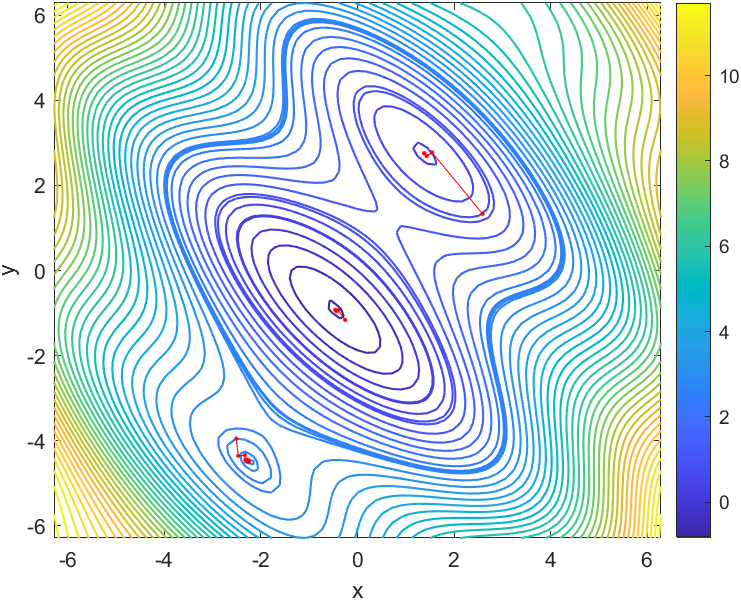
\includegraphics{p1_visualize_in_contour.png}
	
	\label{fig:p1_visualize_in_contour}
\end{figure}

The initial points for gradient descent chosen are $(-3,-4)$, $(0,-1)$, and $(-2,-2)$. The choice of initial points are significant. It can \textbf{influence the speed of convergence dramatically}. Given a bad initial point, the algorithm may not reach the point of convergence at all, or take a unbearable long time to reach there. It worth mentioning that the second choice of $(0,-1)$ is especially difficult. It takes a great many attempts to find this point which contributes to a high speed of convergence.


\begin{table}[h]
	\label{table:p1result}
	\caption{The Extreme Values of $F(x,y)$}
	\begin{center}
		\begin{tabular}{|c|c|c|c|}
			\hline
			No. & X-Y Coordinates & $F(x,y)$ & Result of $fminsearch()$ \\ \hline
			0 & $(-2.2469,-4.4902)$ & 2.5874 &  2.5874 \\ \hline
			1 & $(-0.4611,-0.9241)$ & -0.8549 & -0.8549 \\ \hline
			2 & $(1.3768,2.7529)$ & 0.3020 & 0.3020 \\ \hline
		\end{tabular}
	\end{center}
\end{table}

\subsection{Analysis and Conclusion}   
  

Gradient descent is a widely-used way of finding the extreme values of any function. There are many optimizations for this method, which will improve the speed of convergence. SGD is taken in this project, which yields satisfying results.

SGD gradient descent has a major flaw that it is known for "easy to be trapped in a local minimum", which may account for the difficulties in finding a good initial point for the second extreme value. More sophisticated optimization such as Momentum gradient descent and AdaGrad gradient descent can be applied if the speed of convergence is too slow.



\section{Acknowledgment}

Thanks to (TODO)


\end{document}
